\documentclass[12pt]{article}
\usepackage{amsmath}
\usepackage{graphicx}
\usepackage{hyperref}
\usepackage[utf8]{inputenc}
\usepackage{geometry}
\usepackage{mathtools}
\usepackage{empheq}
\usepackage{listings}
\usepackage{xcolor}
\usepackage{caption}
\usepackage{subcaption}
\usepackage{setspace}
\usepackage{indentfirst}
\usepackage{authblk}
\usepackage{svg}

\graphicspath{ {./} }
\geometry{margin=1in}
\doublespacing
\captionsetup{labelfont=bf}

\title{CHEN 425 Workshop 1}
\author{Mark Levchenko}
\date{25 January 2023}

\begin{document}

% Info %%%%%%%%%%%%%%%%%%%%%%%%%%%%%%%%%%%%%%%%%%%%%%%%%%%%

\textbf{CHEN 425 ASPEN Simulation Report}

\textbf{Title:} Use of the ASPEN RADFRAC Design Spec

\textbf{Workshop:} \#4

\textbf{Date:} February 22, 2023

\textbf{Prepared by:} Mark Levchenko

\textbf{To:} Professor Mahmoud El-Halwagi


% Report %%%%%%%%%%%%%%%%%%%%%%%%%%%%%%%%%%%%%%%%%%%%%%%%%%%%
\section{Summary of Results}
\subsection{Part A}
In order to meet the required distillate and bottoms specifications, the reflux ratio was 1.2037 and the distillate rate was 56504.8 lb/hr. In order to meet these rates, the condenser duty was $5.8383\cdot10^7$ Btu/hr and the reboiler duty was $6.10364\cdot10^7$ Btu/hr.

\subsection{Part B}
In order to meet the required distillate and bottoms specifications with the 65\% efficient trays, the reflux ratio was 1.58658 and the distillate rate was 56504.8 lb/hr. In order to meet these rates, the condenser duty was $6.85269\cdot10^7$ Btu/hr and the reboiler duty was $7.11795\cdot10^7$ Btu/hr.

\subsection{Part C}
\begin{enumerate}
    \item The single section column with sieve trays requires a diameter of 9.86464 ft.
    \item In the two-section column, the diameter of the section below the feed tray is 9.26729 ft, and the diameter of the section above the feed tray is 9.86485 ft. The smaller diameter of the lower section the diameter will save money on the capital costs of the column and the trays.
    \item The packed column is half the height of the column with trays, but its diameter is much larger. The diameter of the packed column is 14.3397 ft. The column itself will be much cheaper; however, packing is much more expensive than trays. The trays may also require less maintenance, and thus will have lower operating costs.
\end{enumerate}


\subsection{Part D}

\section{Discussion of Simulation Results}

\subsection{Part A}
The distillate flow rate combined with the purity of the distillate means that almost all of the Methanol is being recovered in the distillate stream. The condenser and reboiler duties seem reasonably achievable in an industrial setting. The operation of the column can probably be achieved economically provided that the price of methanol is high enough.

\subsection{Part B}
Clearly the efficiency of the stages has a major impact on the operation of the column. The reflux ration had to be increased significantly in order to meet the required purity in the distillate. The flow rate of the distillate is almost identical as a result of the methanol and water specifications. Furthermore, notice that the reboiler and condenser duties increases significantly. As a result, the efficiency of the stages will have a major impact on the operating costs of the column.

\subsection{Part C}
The height of the single section and the two-section column are the same. The diameter of the lower section of the two-section column is less than the diameter of the single section column. The smaller diameter of the lower section of the two-section column will lead to a lower capital cost of the column and the trays as smaller trays will are required.

\subsection{Part D}
The height of the packed column is much smaller which will result in a lower capital cost of the column shell. However, in packed columns, almost the entire inside of the column needs to be filled with material as opposed to columns with trays which only need sheet metal spaced every few feet. The higher material costs combined with the added complexity of packing result in a much higher overall capital cost of installing a packed column. Packed columns also require more work during installation and additional structures inside the column to support the packing and ensure even distribution of the fluid into the packing. However, packing generally is more efficient than trays are, and the increased efficiency can offset the capital costs by lowering operating costs. In the right situation, using packing inside a distillation column can have tremendous benefits.



\section{Simulation Screenshots}

Main flowsheet:
\begin{center}
    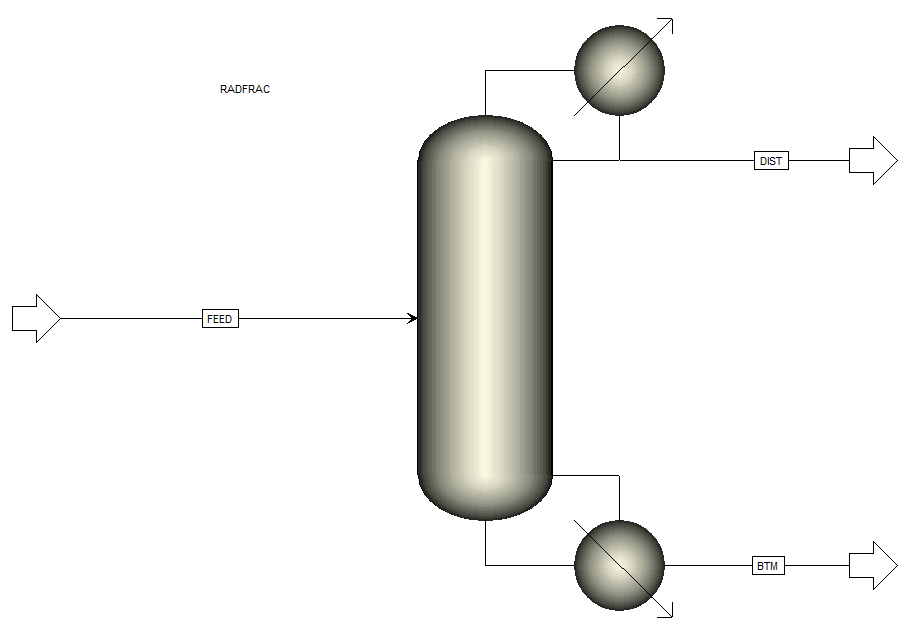
\includegraphics[scale=0.5]{main flowsheet.png}
\end{center}
Part A Reflux ratio Design spec results:
\begin{center}
    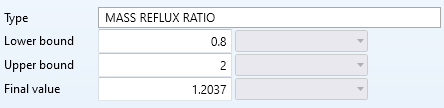
\includegraphics{reflux design spec.png}
\end{center}
Part B Distillate rate design spec results:
\begin{center}
    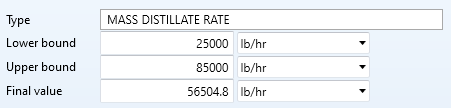
\includegraphics{distillate rate spec.png}
\end{center}
Part B Reflux ratio Design spec results:
\begin{center}
    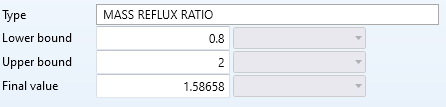
\includegraphics{reflux design spec B.png}
\end{center}
Part B Distillate rate design spec results:
\begin{center}
    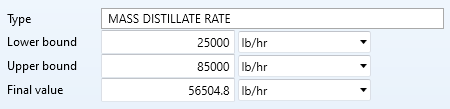
\includegraphics{distillate rate spec B.png}
\end{center}
Stream results showing specification mass fractions:
\begin{center}
    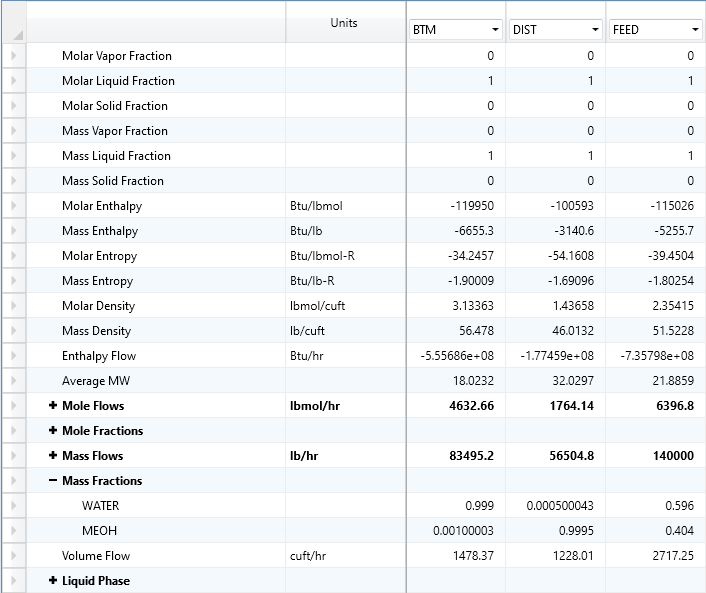
\includegraphics[scale=0.8]{stream results.png}
\end{center}
Part A RADFRAC block results:
\begin{center}
    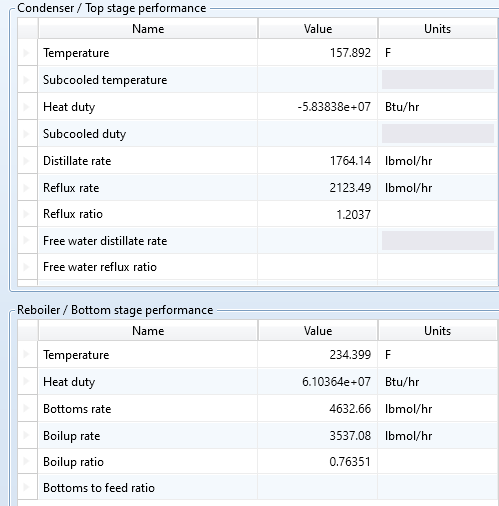
\includegraphics{radfrac results.png}
\end{center}
Part B RADFRAC block results:
\begin{center}
    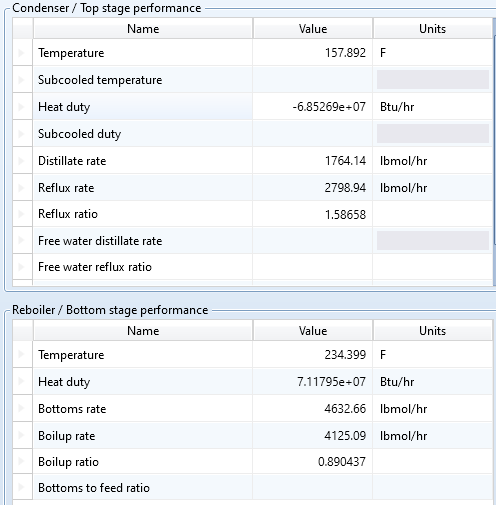
\includegraphics{radfrac results B.png}
\end{center}
Part C Sieve tray results for a uniform diameter:
\begin{center}
    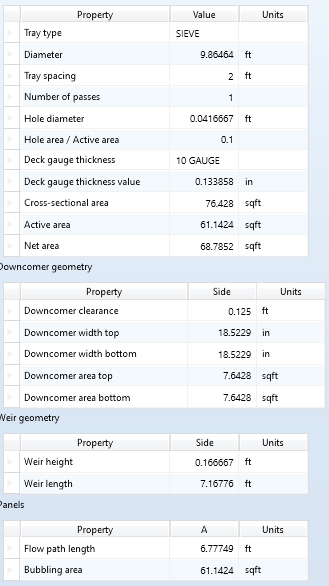
\includegraphics{sieve 1 geometry.png}
    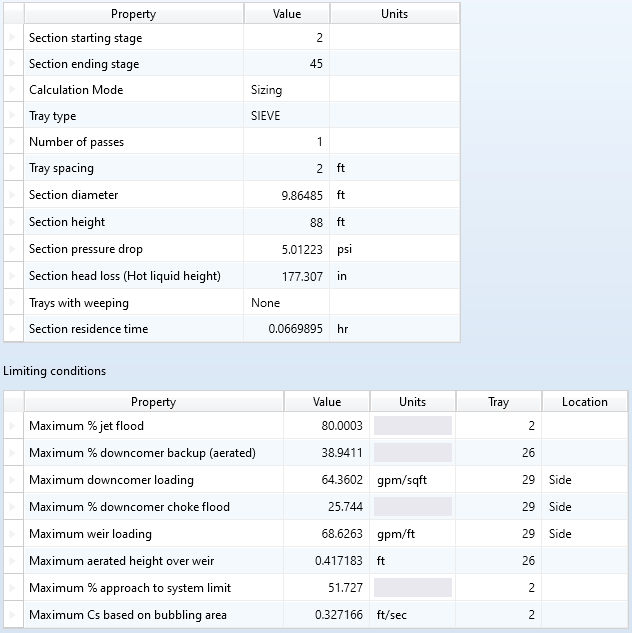
\includegraphics[scale=0.9]{sieve 1 results.png}
\end{center}
Part C Sieve tray results for a two-section column:

Upper section of the column:
\begin{center}
    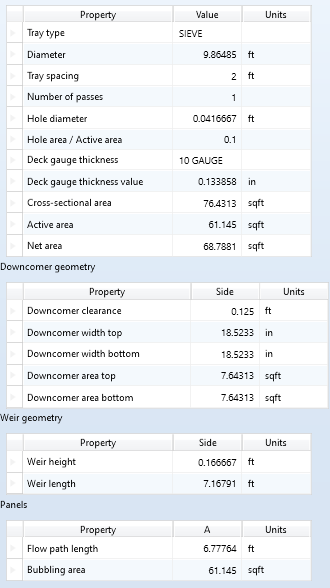
\includegraphics{sieve 2 lower geometry.png}
    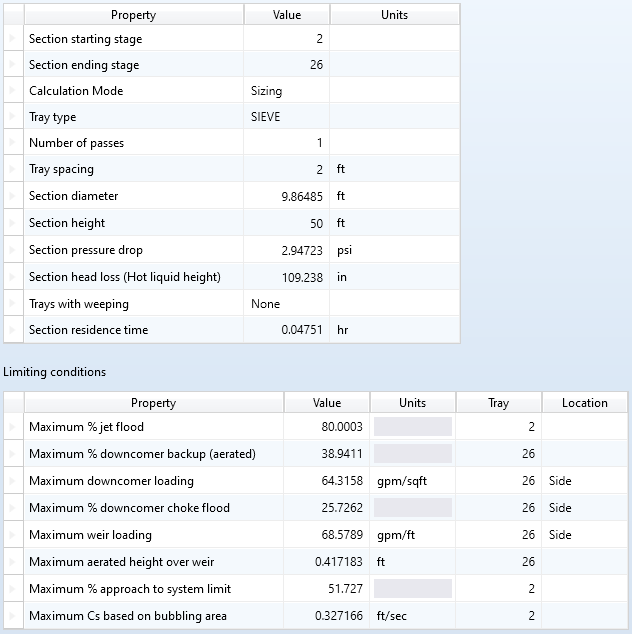
\includegraphics[scale=0.9]{sieve 2 lower results.png}
\end{center}

Lower section of the column:
\begin{center}
    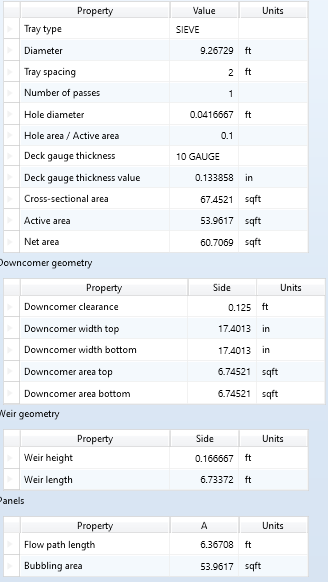
\includegraphics{sieve 2 upper geometry.png}
    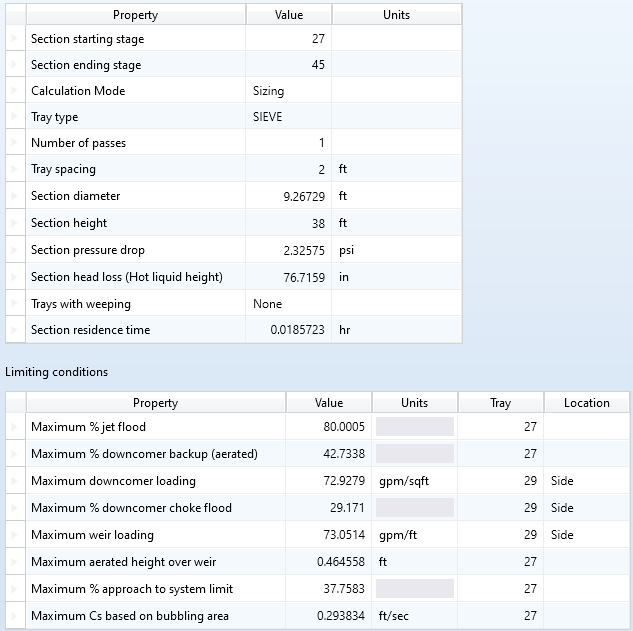
\includegraphics[scale=0.9]{sieve 2 upper results.png}
\end{center}

Part D Packed column results:
\begin{center}
    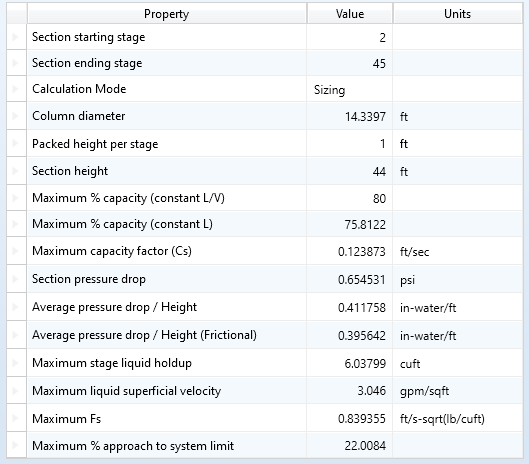
\includegraphics{packing results.png}
\end{center}


\section{Conclusions}

\end{document}